\section{Quadrature}

The central building block for evaluating inner products is the calculation of
integrals between wavepackets.
This is done numerically with a quadrature rule, of which there are many
different kinds.

\subsection{Gauss-Hermite Quadrature}

The basic integration algorithm used in this project is the one-dimensional
Gauss-Hermite quadrature.
Like related rules, this method works by evaluating the integrand function at a
defined set of nodes $\gamma_i$, the values of which are summed up with specific
weights $\omega_i$:

\begin{equation}
  \label{eq:gaussquad}
  \int_{-\infty}^{\infty} g(x) \, dx \approx \sum_{i=1}^{n} f(\gamma_i) \omega_i
\end{equation}

In its basic form, the Gauss-Hermite rule works on special integrals of the
following form:

\begin{equation}
  \int_{-\infty}^{\infty} e^{-x^2} f(x) \, dx
\end{equation}

However, as we require the quadrature to work on general functions,
transformations are done to the usual weights and nodes which is described in
\cite{B_master_thesis}.
The result is a rule in the form of \eqref{eq:gaussquad}.
Figure~\ref{fig:ghexample} shows an example of the node distribution of a
Gauss-Hermite rule.

\begin{figure}
  \center
  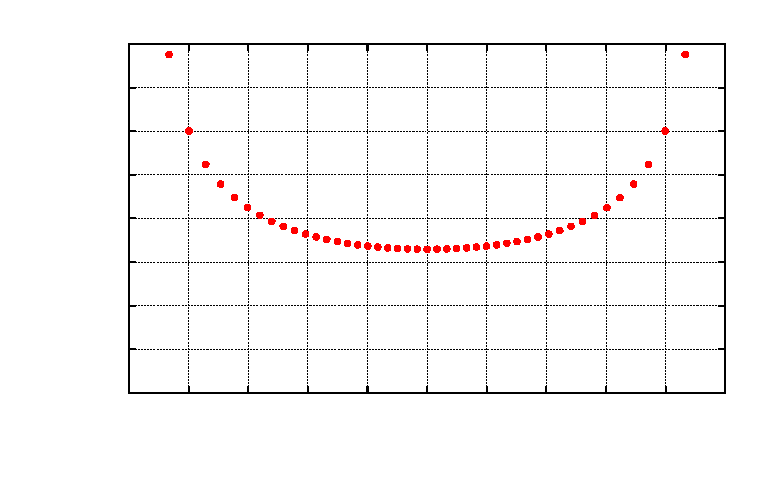
\includegraphics[width=\linewidth]{figures/gh-rule.eps}
  \caption{45-point Gauss-Hermite nodes and weights}
  \label{fig:ghexample}
\end{figure}
